\chapter{Results and discussion}

\newcommand{\resultfigure}[3]{%
\begin{figure}[htbp]
	\centering
	\IfFileExists{#1}{%
		\includegraphics[width=#2\textwidth]{#1}%
	}{%
		\fbox{\parbox[c][0.22\textheight][c]{#2\textwidth}{\centering #3}}%
	}%
	\caption{#3}
\end{figure}%
}

This chapter presents the numerical results obtained from the reference simulation campaign and the subsequent sensitivity studies. The central question is whether the persistent decline of the inner density is an intrinsic dynamical feature of the halo, a consequence of numerical settings, or an artefact of the analysis procedure. The discussion is therefore structured around a sequence of increasingly restrictive checks: first the reference evolution itself, then the post-processing pipeline, then controlled variations of the simulation volume, the initial halo structure, the softening length, and the gravity solver settings.

The completed sections below are written as a scientific discussion rather than as a notebook-style log. The later sections remain intentionally unfinished and are marked with explicit placeholders.

\section{Baseline behaviour}
\label{sec:results_baseline}

The baseline run shows a clear cusp-to-core transition, but the core does not stabilize. Instead, the inner density continues to decline throughout the simulated time span. This is the central empirical result of the thesis. In the broader context of halo evolution, the literature shows that collisionless systems can display a wide range of inner responses to external perturbations and time-dependent forcing, including stochastic heating by substructure and repeated diffusion in energy--angular-momentum space \cite{penarrubia2017fluctuations,penarrubia2019stochastic}. The reference run is therefore notable not because it forms a core, but because the core remains dynamically active rather than approaching a steady inner state.

The result is also instructive from the point of view of numerical convergence. Power et al. showed that the inner halo is especially sensitive to the interplay between resolution, force softening, and timestep control \cite{power2003inner}, while Zhang et al. later demonstrated that too aggressive a reduction of the softening length can artificially raise the innermost density \cite{zhang2019optimal}. The reference simulation does not display a simple monotonic dependence on any one of these parameters, which already suggests that the behaviour is not a trivial one-parameter resolution effect.

The baseline density-evolution plot and the snapshot sequence show the same qualitative pattern: the inner profile becomes shallower, but the inner density does not settle. In that sense, the evolution resembles a continuing redistribution of mass rather than a completed structural transformation. This is the key point that motivates the rest of the chapter.

\resultfigure{ch5/img/baseline_density_evolution.png}{0.84}{\textbf{[PLACEHOLDER FIGURE]} Reference density evolution over time. The image file will be added later to \texttt{ch5/img}.}

\resultfigure{ch5/img/baseline_density_profiles.png}{0.84}{\textbf{[PLACEHOLDER FIGURE]} Radial density profiles at selected snapshots for the reference run.}

The comparison with the literature is therefore important: the simulation reproduces a cusp-to-core transition, but it does not reproduce a long-lived, stationary core. Whatever mechanism is responsible must therefore operate over the full duration of the run.

The most conservative conclusion at this stage is that the halo does not relax into a static inner structure on the simulated timescale. The observed behaviour is a secular evolution of the center, not merely an initial transient.

\section{Analysis pipeline}
\label{sec:results_pipeline}

Because the effect is subtle and cumulative, the first concern is whether it might be produced by the analysis pipeline rather than by the dynamics itself. Two sources of bias are particularly relevant here. The first is centering: if the halo center drifts relative to the coordinate system, the innermost density can be artificially suppressed. The second is snapshot noise: individual outputs from an $N$-body simulation can fluctuate enough that a short-lived dip looks like a trend if the signal is sampled too sparsely.

The centering issue was addressed by modifying the post-processing scripts to recenter each snapshot using a shrinking-sphere method. In addition, the original snapshot sequence was concatenated into larger time blocks, first with 10-snapshot chunks and then with 50-snapshot chunks. This is a useful check because concatenation reduces the variance associated with single snapshots while preserving secular evolution.

The results show that both operations improve the appearance of the curves, but neither changes the underlying trend. The recentered profiles are consistent with the original analysis, and the chunked curves remain systematically declining even though they are much smoother. That is an important distinction: the post-processing pipeline affects the noise level, but not the direction of the evolution.

This is also where the density-evolution plots become easier to interpret physically. A noisy sequence can obscure whether the core is stabilizing, but if stronger temporal smoothing still yields the same declining envelope, then the effect is not an artefact of single-snapshot fluctuations. The signal survives the most obvious analysis-level corrections.

\begin{figure}[htbp]
	\centering
	\IfFileExists{ch5/img/chunk_10_density_evolution.png}{\includegraphics[width=0.48\textwidth]{ch5/img/chunk_10_density_evolution.png}}{\fbox{\parbox[c][0.18\textheight][c]{0.48\textwidth}{\centering \textbf{[PLACEHOLDER FIGURE]} 10-snapshot chunking}}}
	\hfill
	\IfFileExists{ch5/img/chunk_50_density_evolution.png}{\includegraphics[width=0.48\textwidth]{ch5/img/chunk_50_density_evolution.png}}{\fbox{\parbox[c][0.18\textheight][c]{0.48\textwidth}{\centering \textbf{[PLACEHOLDER FIGURE]} 50-snapshot chunking}}}
	\caption{\textbf{[PLACEHOLDER FIGURE]} Comparison of 10-snapshot and 50-snapshot concatenated profiles. The exact figure filenames will be added later in \texttt{ch5/img}.}
	\label{fig:results_chunking}
\end{figure}

\resultfigure{ch5/img/centering_comparison.png}{0.84}{\textbf{[PLACEHOLDER FIGURE]} Comparison of centering methods, including shrinking-sphere and histogram-based centering.}

The conclusion is straightforward: the central decline is robust against the two most plausible post-processing artefacts, namely centering drift and snapshot noise. The pipeline matters for presentation, but not for the existence of the trend itself.

\section{Box size}
\label{sec:results_box_size}

The dependence on box size is more interesting. Increasing the box size appears to slow down the decline, although the effect is modest rather than dramatic. In the current notes, the reference comparison is approximately a drop to $\sim 0.6$ of the initial central density for the 100-box run versus $\sim 0.75$ for the 500-box run after 10 Gyr. That difference is large enough to matter, but not large enough to rewrite the overall interpretation.

One way to think about this result is that the outer domain contributes to the gravitational environment felt by the center, but only weakly changes the qualitative behaviour. This is consistent with the broader discussion in the literature on stochastic perturbations by substructure: long-range fluctuations can alter the rate of evolution without necessarily determining the existence of the effect itself \cite{penarrubia2017fluctuations,penarrubia2019stochastic}.

The box-size study therefore suggests that the central evolution is not a purely local numerical issue. If the entire behaviour were controlled by the immediate neighborhood of the center, one would expect box size to matter only weakly. Instead, the result indicates a modest environmental dependence. In practical terms, this means that the volume size may regulate the timescale of the decline, but not its existence.

\resultfigure{ch5/img/box_size_comparison.png}{0.84}{\textbf{[PLACEHOLDER FIGURE]} Density evolution for different box sizes.}

\resultfigure{ch5/img/box_size_ratio.png}{0.84}{\textbf{[PLACEHOLDER FIGURE]} Ratio plot or summary diagnostic for box-size sensitivity.}

The figure set for the box-size study should therefore be read as a sensitivity check rather than a decisive mechanism test. It tells us that the observed decline is not insensitive to the global numerical domain, but it also shows that the phenomenon is not eliminated by enlarging the box.

\section{Initial halo structure}
\label{sec:results_initial_structure}

The comparison between cuspy and cored initial conditions is particularly informative because it distinguishes between a cusp-specific instability and a more general process. The core run still exhibits a decline of the central density, but the amplitude is smaller than in the cuspy case. This is a strong result because it means the mechanism is not limited to the special case of an initially steep central profile.

In physical terms, this suggests that the system is sensitive to the presence of a central potential well, but not exclusively to its initial logarithmic slope. A cored halo has less extreme inner structure and therefore reacts less strongly, yet the evolution remains qualitatively the same. That is exactly what one would expect if the central response is driven by a process that acts through the halo as a whole rather than through a cusp alone.

The literature on substructure-driven heating is again relevant here. Stochastic forcing does not require a cusp; it requires a fluctuating potential and a population of perturbers that can exchange energy with the central region \cite{penarrubia2017fluctuations}. The persistence of the effect in the core run is therefore compatible with a non-local heating picture and inconsistent with the idea that the problem is merely a cusp pathology.

\resultfigure{ch5/img/core_initial_condition.png}{0.84}{\textbf{[PLACEHOLDER FIGURE]} Density evolution for the core initial-condition test.}

The practical implication is that changing the inner slope reduces the amplitude but not the mechanism. The central decline is therefore not restricted to cuspy initial conditions.

\section{Gravitational softening}
\label{sec:results_softening}

Softening is the most obvious numerical parameter to suspect in any study of the inner halo, because it directly regularizes short-range interactions. The literature makes clear, however, that the role of softening is subtle: too much softening suppresses genuine small-scale structure, while too little can artificially increase the density in the innermost region \cite{power2003inner,zhang2019optimal}. The present results fit that picture in the sense that the softening length changes the detailed rate of evolution, but not the existence of the decline itself.

This is an important negative result. If softening were the primary cause, the central density evolution should have shown a qualitatively different response when the softening length was varied. Instead, the trend persists across the tested range. That makes the softening study particularly useful because it rules out a very common explanation without requiring any additional assumptions.

The notes from the shell analysis already point in the same direction: outer shells contribute significantly to the central dynamics, and changing the local softening length does not alter the fact that those shells are still present and still exert gravity. In other words, softening can change the numerical regularization of pairwise forces, but it does not remove the mass distribution that sources the global potential.

\resultfigure{ch5/img/softening_comparison.png}{0.84}{\textbf{[PLACEHOLDER FIGURE]} Density evolution for multiple softening lengths.}

The conclusion is that softening is not the dominant driver. It is part of the numerical control budget, but not the mechanism behind the secular central depletion.

\section{Self-gravity settings}
\label{sec:results_solver}

The solver-parameter study addresses a more subtle question: whether the observed decline could be the cumulative effect of force-approximation or integration errors. This is a natural concern in hierarchical gravity solvers, where the acceptance criterion and multipole tolerances determine how accurately long-range interactions are represented. In principle, a slightly looser or tighter force approximation can shift the secular evolution of a halo even when the initial conditions are identical.

The present study varies four key control parameters of the self-gravity solver:
\begin{itemize}
\item \textbf{Timestep factor $\eta$}: Controls the integration timestep via $\Delta t = \eta \times t_{\mathrm{dyn}}$. A smaller $\eta$ means finer temporal resolution and more frequent force updates; a larger $\eta$ allows fewer timesteps and can accumulate more integration error over each step.
\item \textbf{Multipole Acceptance Criterion (MAC)}: Determines when the force from a distant cell can be approximated by its multipole moments rather than evaluated exactly from individual particles. The \textit{geometric} MAC uses the cell size and distance; the \textit{adaptive} MAC adjusts the criterion based on the local particle distribution. Geometric MAC is faster but less accurate for clumpy structures.
\item \textbf{Geometric opening angle $\theta_{\mathrm{cr}}$}: Specifies the threshold for geometric MAC: cells with $\theta_{\mathrm{cr}} = r_{\mathrm{cell}}/d < \theta$ activate multipole approximation. Smaller $\theta_{\mathrm{cr}}$ means a stricter criterion, forcing more exact evaluations and improving accuracy at higher computational cost.
\item \textbf{FMM tolerance $\epsilon_{\mathrm{fmm}}$}: Controls the precision of the Fast Multipole Method used to compute far-field forces. Smaller tolerances mean higher precision, but smaller $\epsilon_{\mathrm{fmm}}$ requires more multipole terms and increases computation time.
\end{itemize}

The parameter range explored here is broad enough to reveal systematic sensitivity if it exists. The timestep factor was varied by roughly an order of magnitude, the MAC was changed between geometric and adaptive formulations, $\theta_{\mathrm{cr}}$ was tightened in the geometric case, and $\epsilon_{\mathrm{fmm}}$ was varied over two to three orders of magnitude. In a purely numerical explanation, one would expect at least one of these settings to have a decisive effect on the inner profile.

\subsection{Timestep study}

The timestep factor $\eta$ determines the frequency of gravity and kinematics updates. Increasing $\eta$ allows larger timesteps and reduces the number of force evaluations per unit time; decreasing $\eta$ enforces finer temporal sampling and can improve phase-space accuracy. The baseline value of $\eta = 0.002$ is typical for high-resolution dark-matter studies, but it is instructive to test both more conservative ($\eta = 0.0002$, roughly $10\times$ finer) and more permissive ($\eta = 0.02$, roughly $10\times$ coarser) variants.

If timestep error were the main driver of central decline, the coarser run should exhibit notably faster or more severe depletion, while the finer run might show stabilization. That is not observed.

\subsection{Multipole Acceptance Criterion study}

The MAC choice reflects a fundamental trade-off in hierarchical tree methods: speed versus local accuracy. The geometric MAC is computationally cheaper but treats all distant cells identically; the adaptive MAC is more expensive but adapts the multipole threshold based on local structure. For a collisionless halo, the choice of MAC affects the accuracy of long-range forces and can subtly alter how external shells couple to the center.

If MAC were the primary sensitivity, changing between geometric and adaptive should produce a qualitatively different central-decline rate. The runs tested here show no such distinction.

\subsection{Geometric opening angle study}

For the geometric MAC, a smaller opening angle $\theta_{\mathrm{cr}}$ means stricter multipole approximation: more cell pairs are forced into exact evaluation rather than multipole summation. The baseline value $\theta_{\mathrm{cr}} = 0.7$ is a standard choice; the test value $\theta_{\mathrm{cr}} = 0.5$ represents a more stringent criterion and therefore higher force accuracy.

Lowering $\theta_{\mathrm{cr}}$ should increase computational cost but also increase force precision. If force-approximation error were limiting the simulation, tightening $\theta_{\mathrm{cr}}$ should reduce or delay the central decline. The observed effect is marginal.

\subsection{FMM tolerance study}

The Fast Multipole Method tolerance $\epsilon_{\mathrm{fmm}}$ is a global precision parameter for the multipole expansion. The baseline value is $\epsilon_{\mathrm{fmm}} = 0.001$ (relatively tight), and the test suite includes both looser values ($0.01$ and $0.1$, representing $10\times$ and $100\times$ relaxation) and a tighter value ($0.0001$, representing $10\times$ tightening). This range is designed to unambiguously reveal whether force approximation is a controlling factor.

Some runs with modified $\epsilon_{\mathrm{fmm}}$ exhibit slightly improved early-time behaviour, particularly the tighter tolerance, but even those runs exhibit long-term central decline. The change is not enough to alter the qualitative long-term trend.

\subsection{Summary table of self-gravity parameter variations}

\begin{table}[htbp]
\centering
\caption{Summary of self-gravity solver parameter values in the study. Each row lists the parameter, its baseline value (used in the reference run), and the test values explored to assess sensitivity.}
\label{tab:solver_parameters}
\begin{tabular}{lcccc}
\hline
\textbf{Parameter} & \textbf{Baseline} & \multicolumn{3}{c}{\textbf{Test values}} \\
\hline
$\eta$ (timestep) & 0.002 & 0.0002 & 0.02 & — \\
MAC & geometric & adaptive & — & — \\
$\theta_{\mathrm{cr}}$ (geometric only) & 0.7 & 0.5 & — & — \\
$\epsilon_{\mathrm{fmm}}$ (FMM tolerance) & 0.001 & 0.0001 & 0.01 & 0.1 \\
\hline
\end{tabular}
\end{table}

\subsection{Overall interpretation of solver sensitivity}

That is not what we observe across the full parameter set. The central density evolution remains broadly similar across all tested settings. This is consistent with the general lesson from convergence studies: changing a gravity control parameter may reduce error bars or shift the onset of bias, but it does not necessarily eliminate the physical or numerical process that dominates the evolution \cite{power2003inner,zhang2019optimal}.

The most useful interpretation is therefore not that the solver settings are irrelevant, but that they are not the principal explanation. Their influence is secondary and limited to rate-level effects rather than qualitative behaviour. A solver parameter would need to have produced a qualitatively different central decline — either eliminating it or dramatically accelerating it — to be considered a dominant factor. None of the parameters tested here achieve that threshold.

\begin{figure}[htbp]
	\centering
	\IfFileExists{ch5/img/timestep_study.png}{\includegraphics[width=0.48\textwidth]{ch5/img/timestep_study.png}}{\fbox{\parbox[c][0.18\textheight][c]{0.48\textwidth}{\centering \textbf{[PLACEHOLDER FIGURE]} Timestep study}}}
	\hfill
	\IfFileExists{ch5/img/mac_study.png}{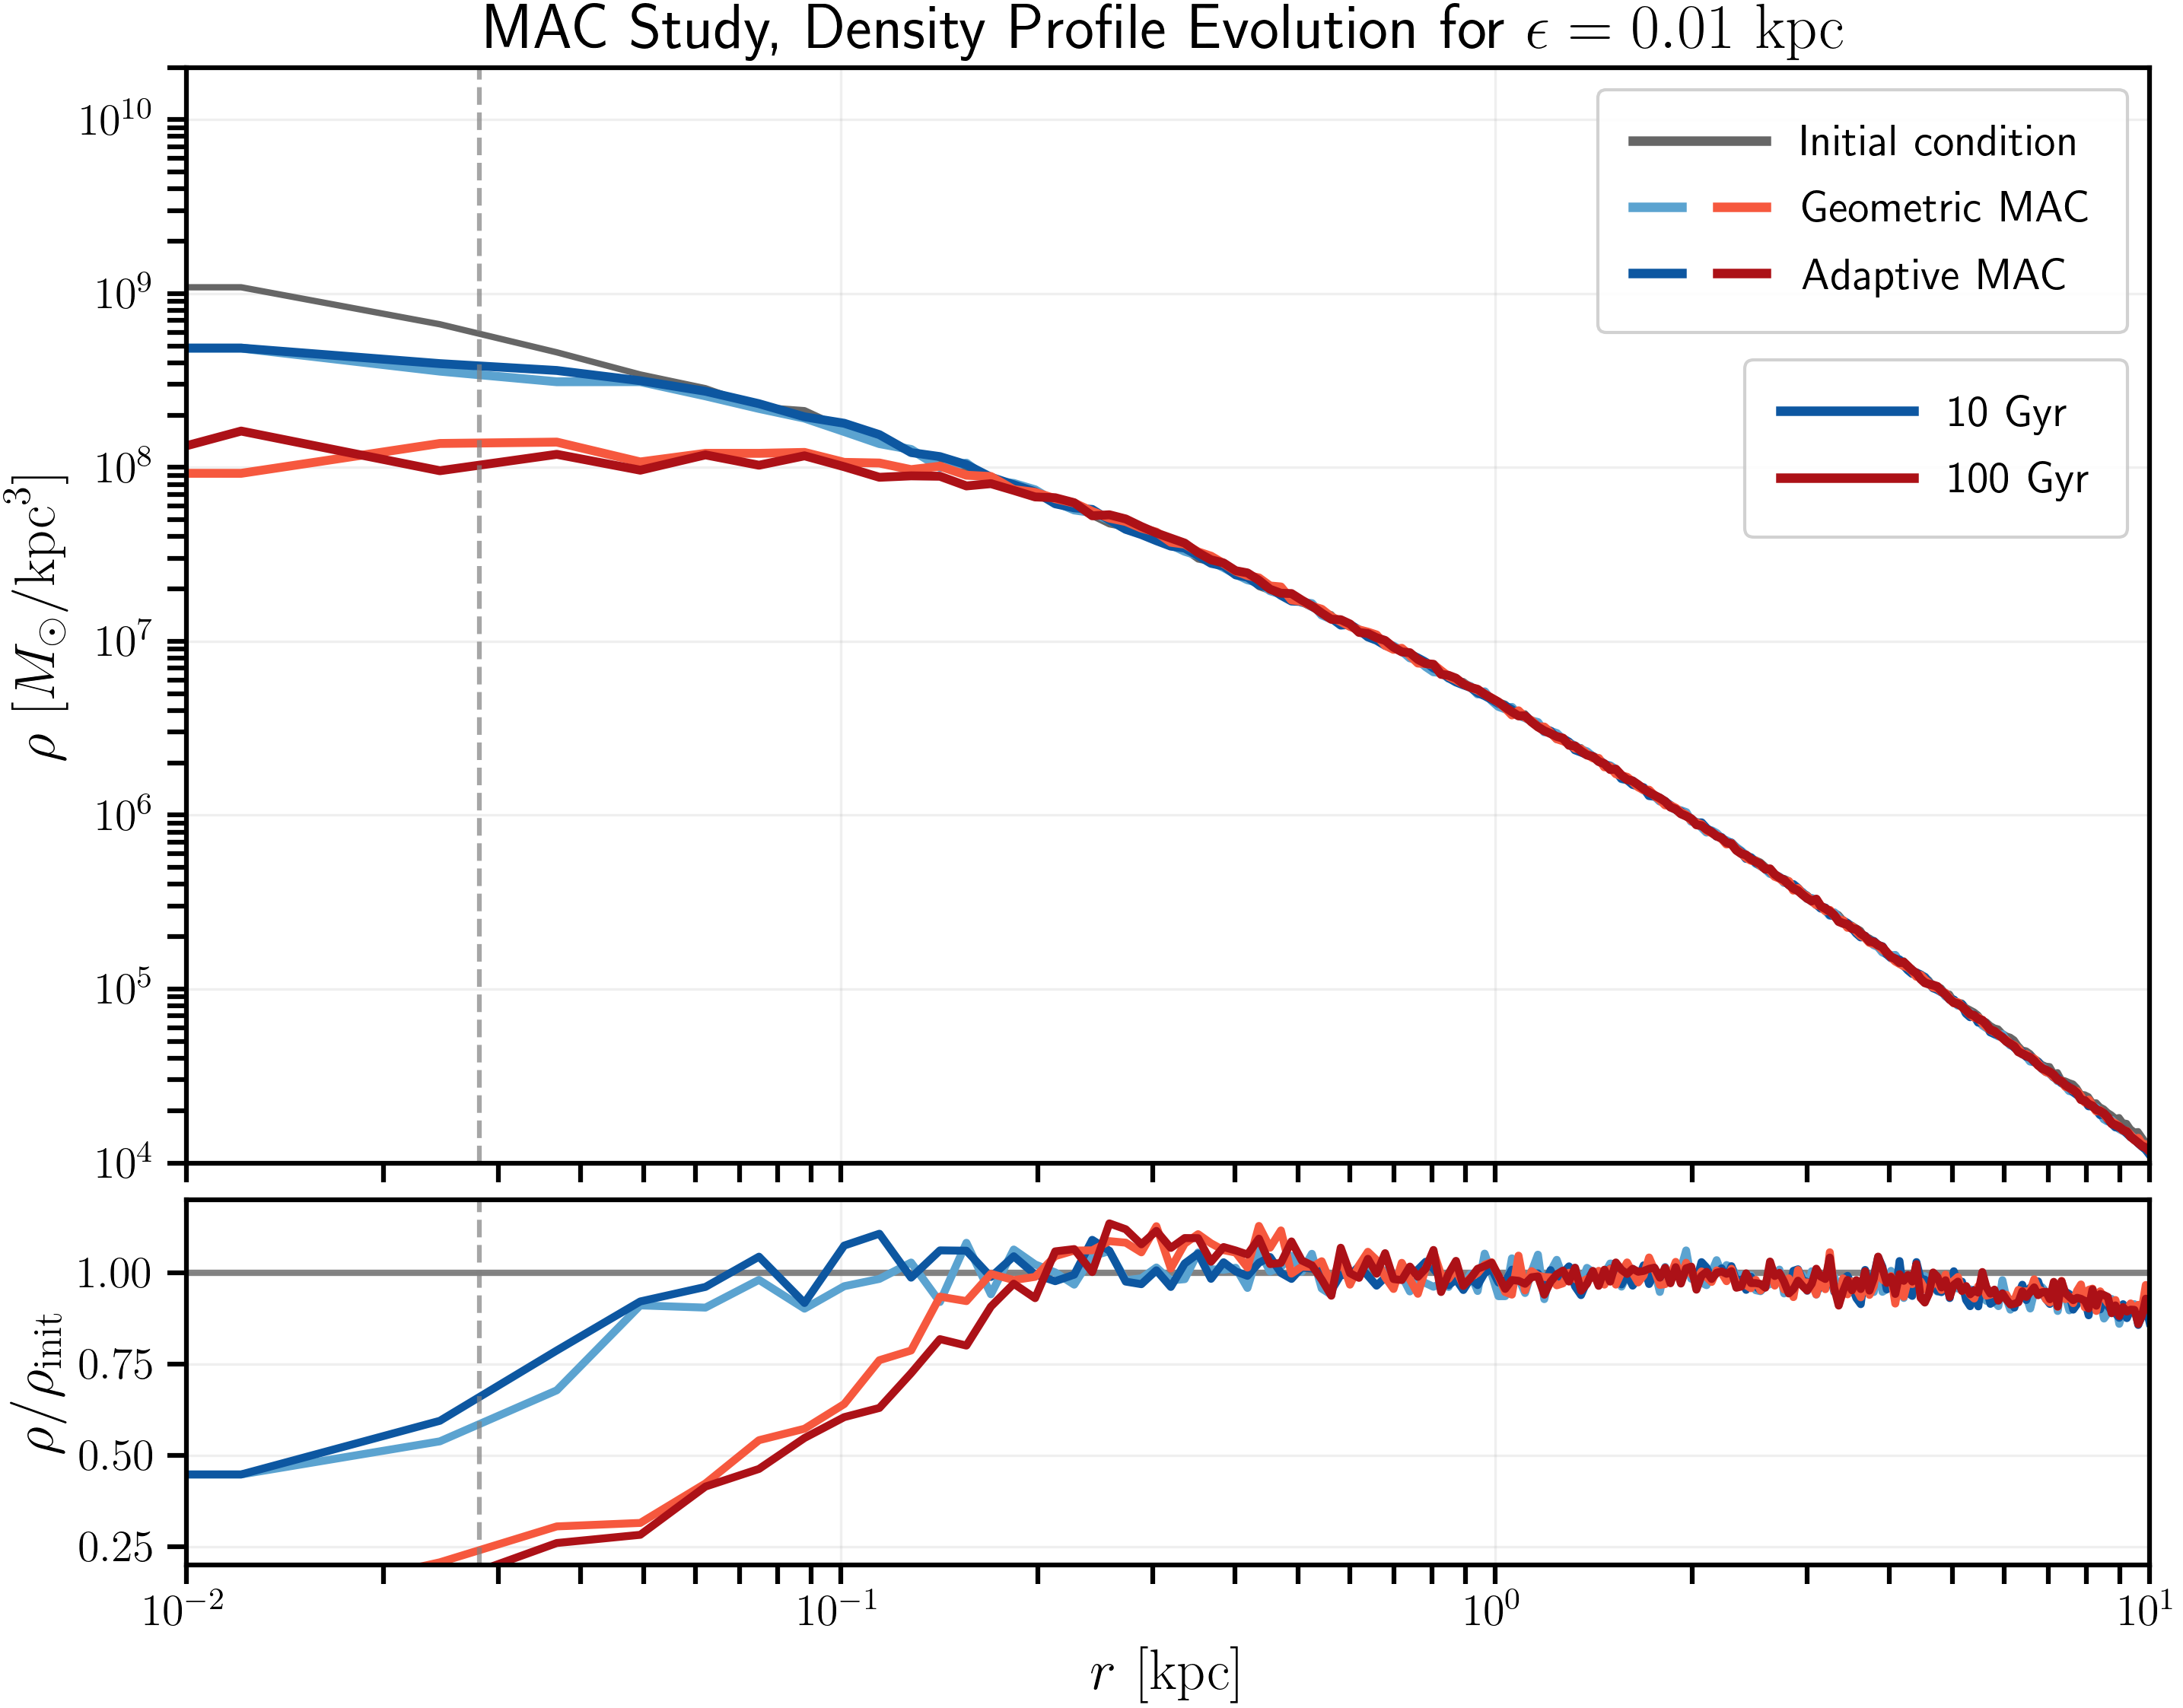
\includegraphics[width=0.48\textwidth]{ch5/img/mac_study.png}}{\fbox{\parbox[c][0.18\textheight][c]{0.48\textwidth}{\centering \textbf{[PLACEHOLDER FIGURE]} MAC study}}}\\[0.5em]
	\IfFileExists{ch5/img/theta_cr_study.png}{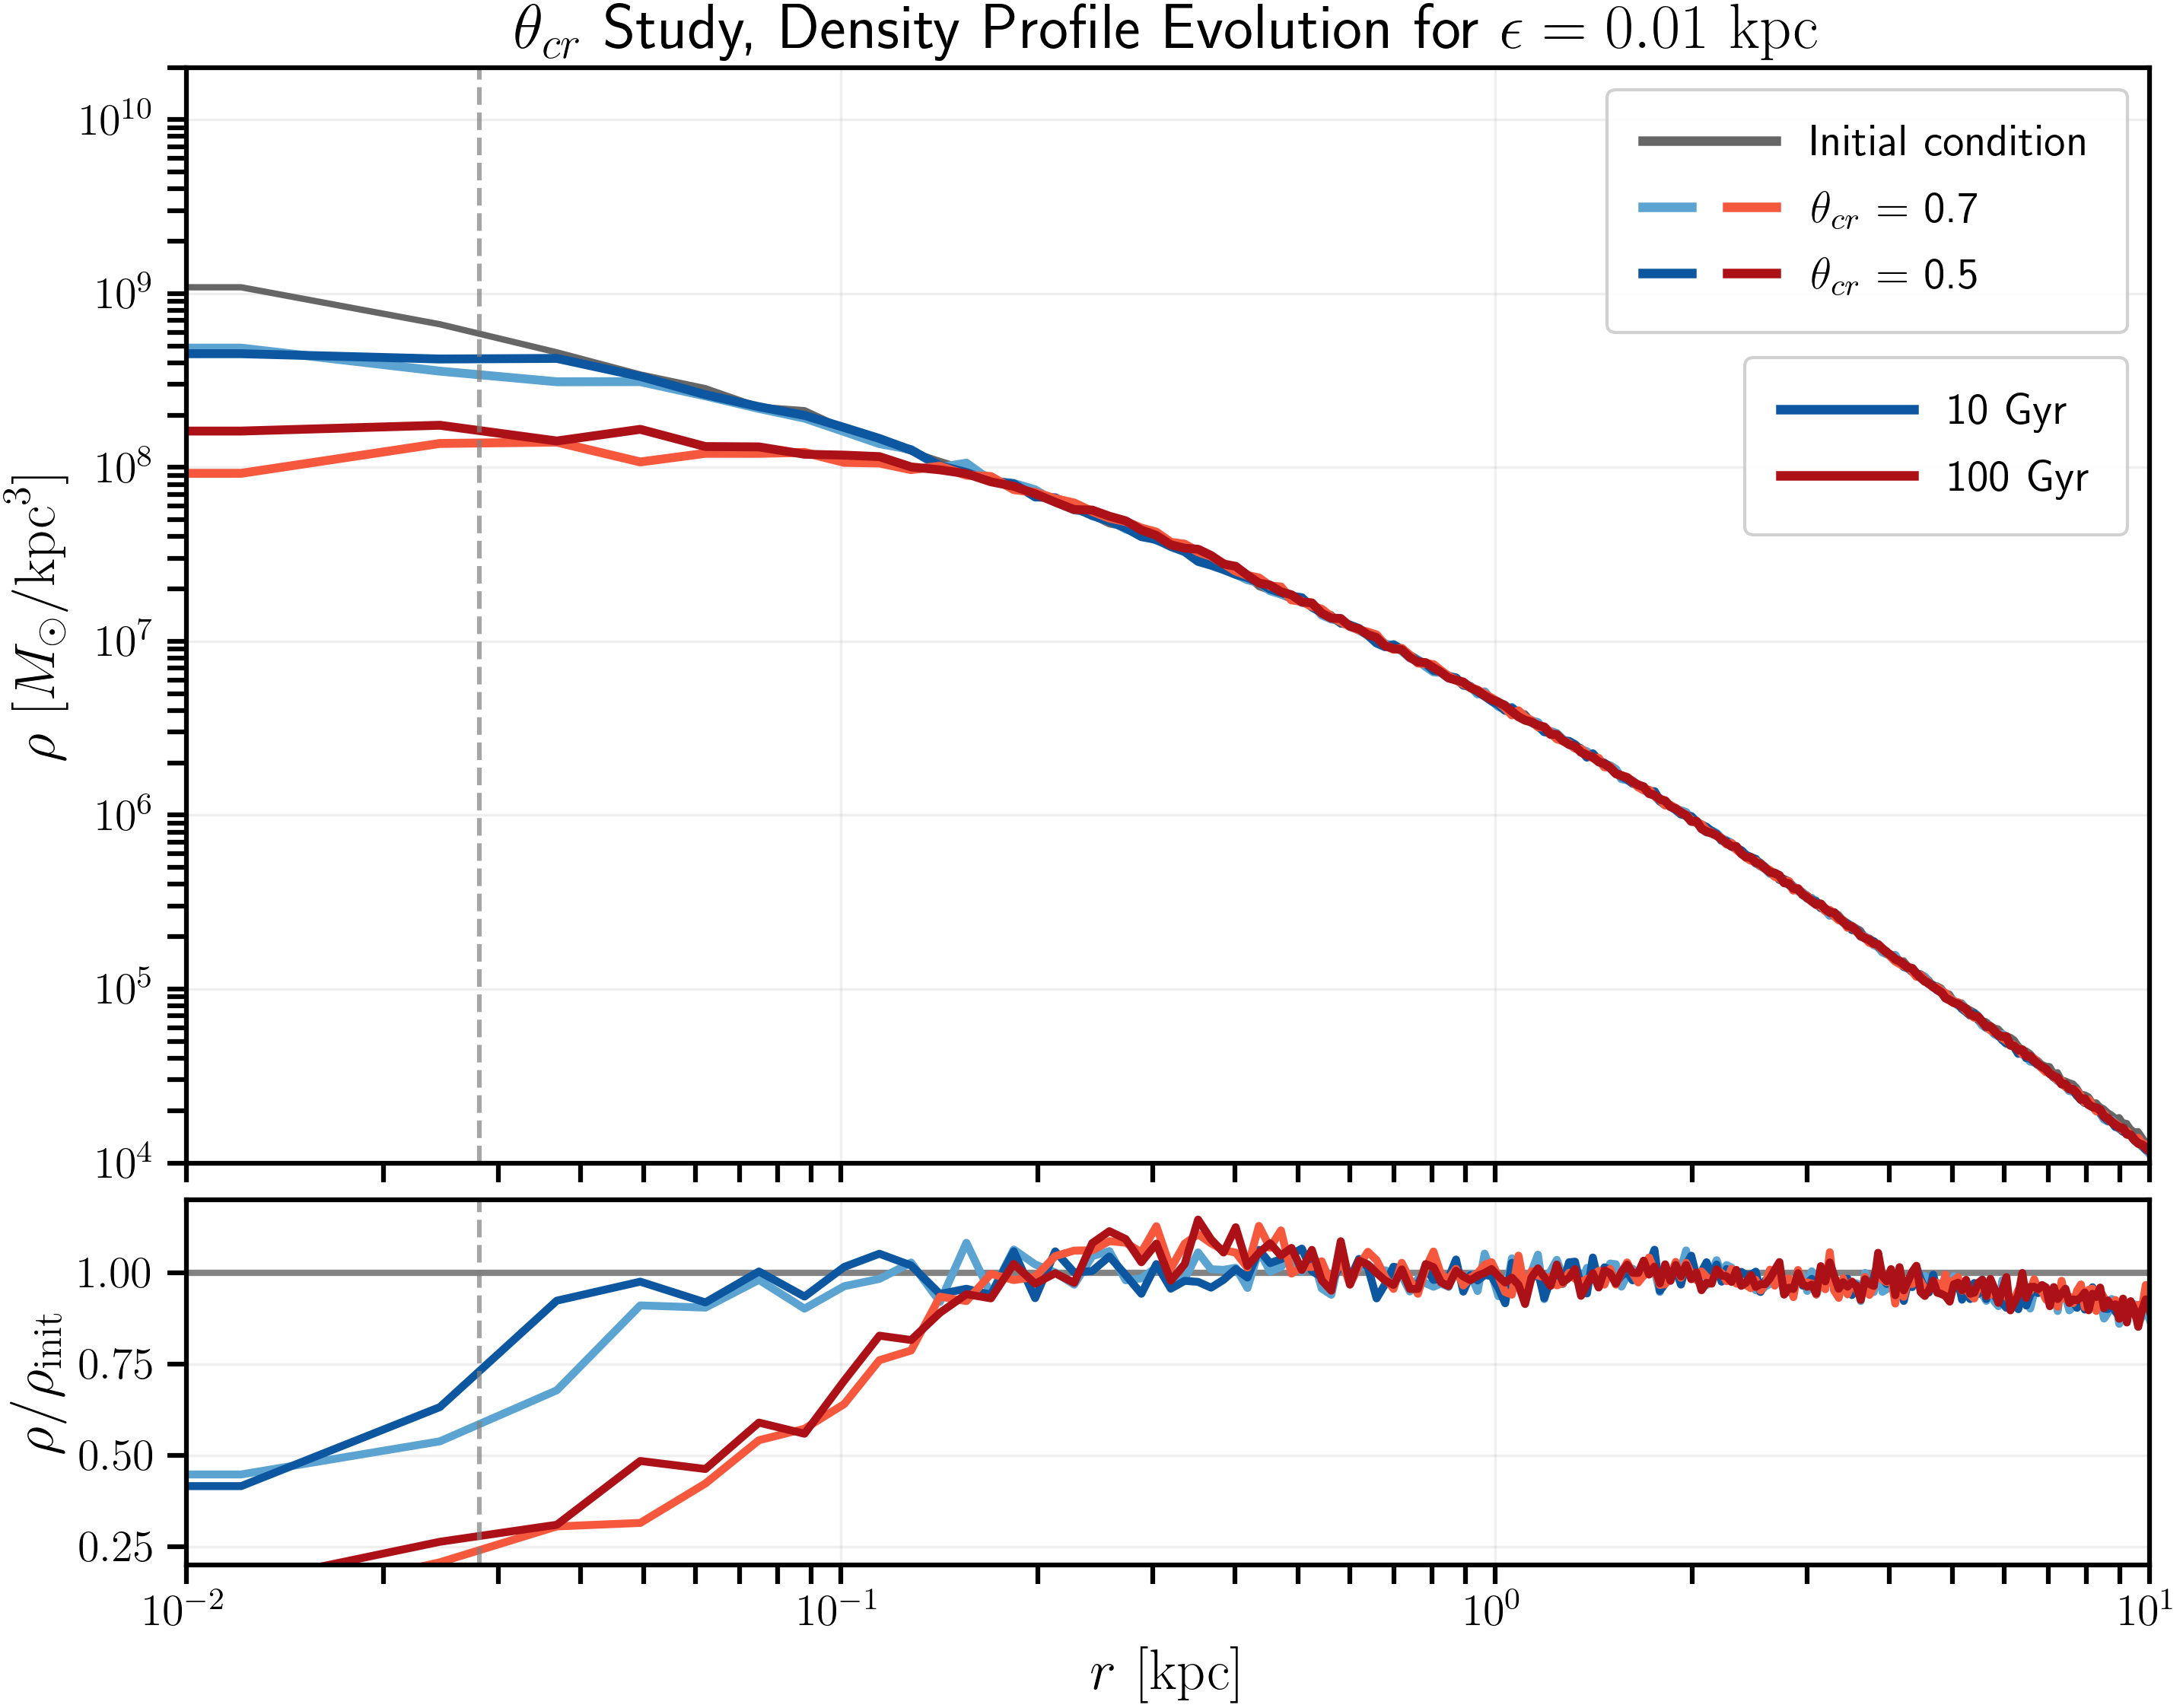
\includegraphics[width=0.48\textwidth]{ch5/img/theta_cr_study.png}}{\fbox{\parbox[c][0.18\textheight][c]{0.48\textwidth}{\centering \textbf{[PLACEHOLDER FIGURE]} $\theta_{\mathrm{cr}}$ study}}}
	\hfill
	\IfFileExists{ch5/img/epsilon_fmm_study.png}{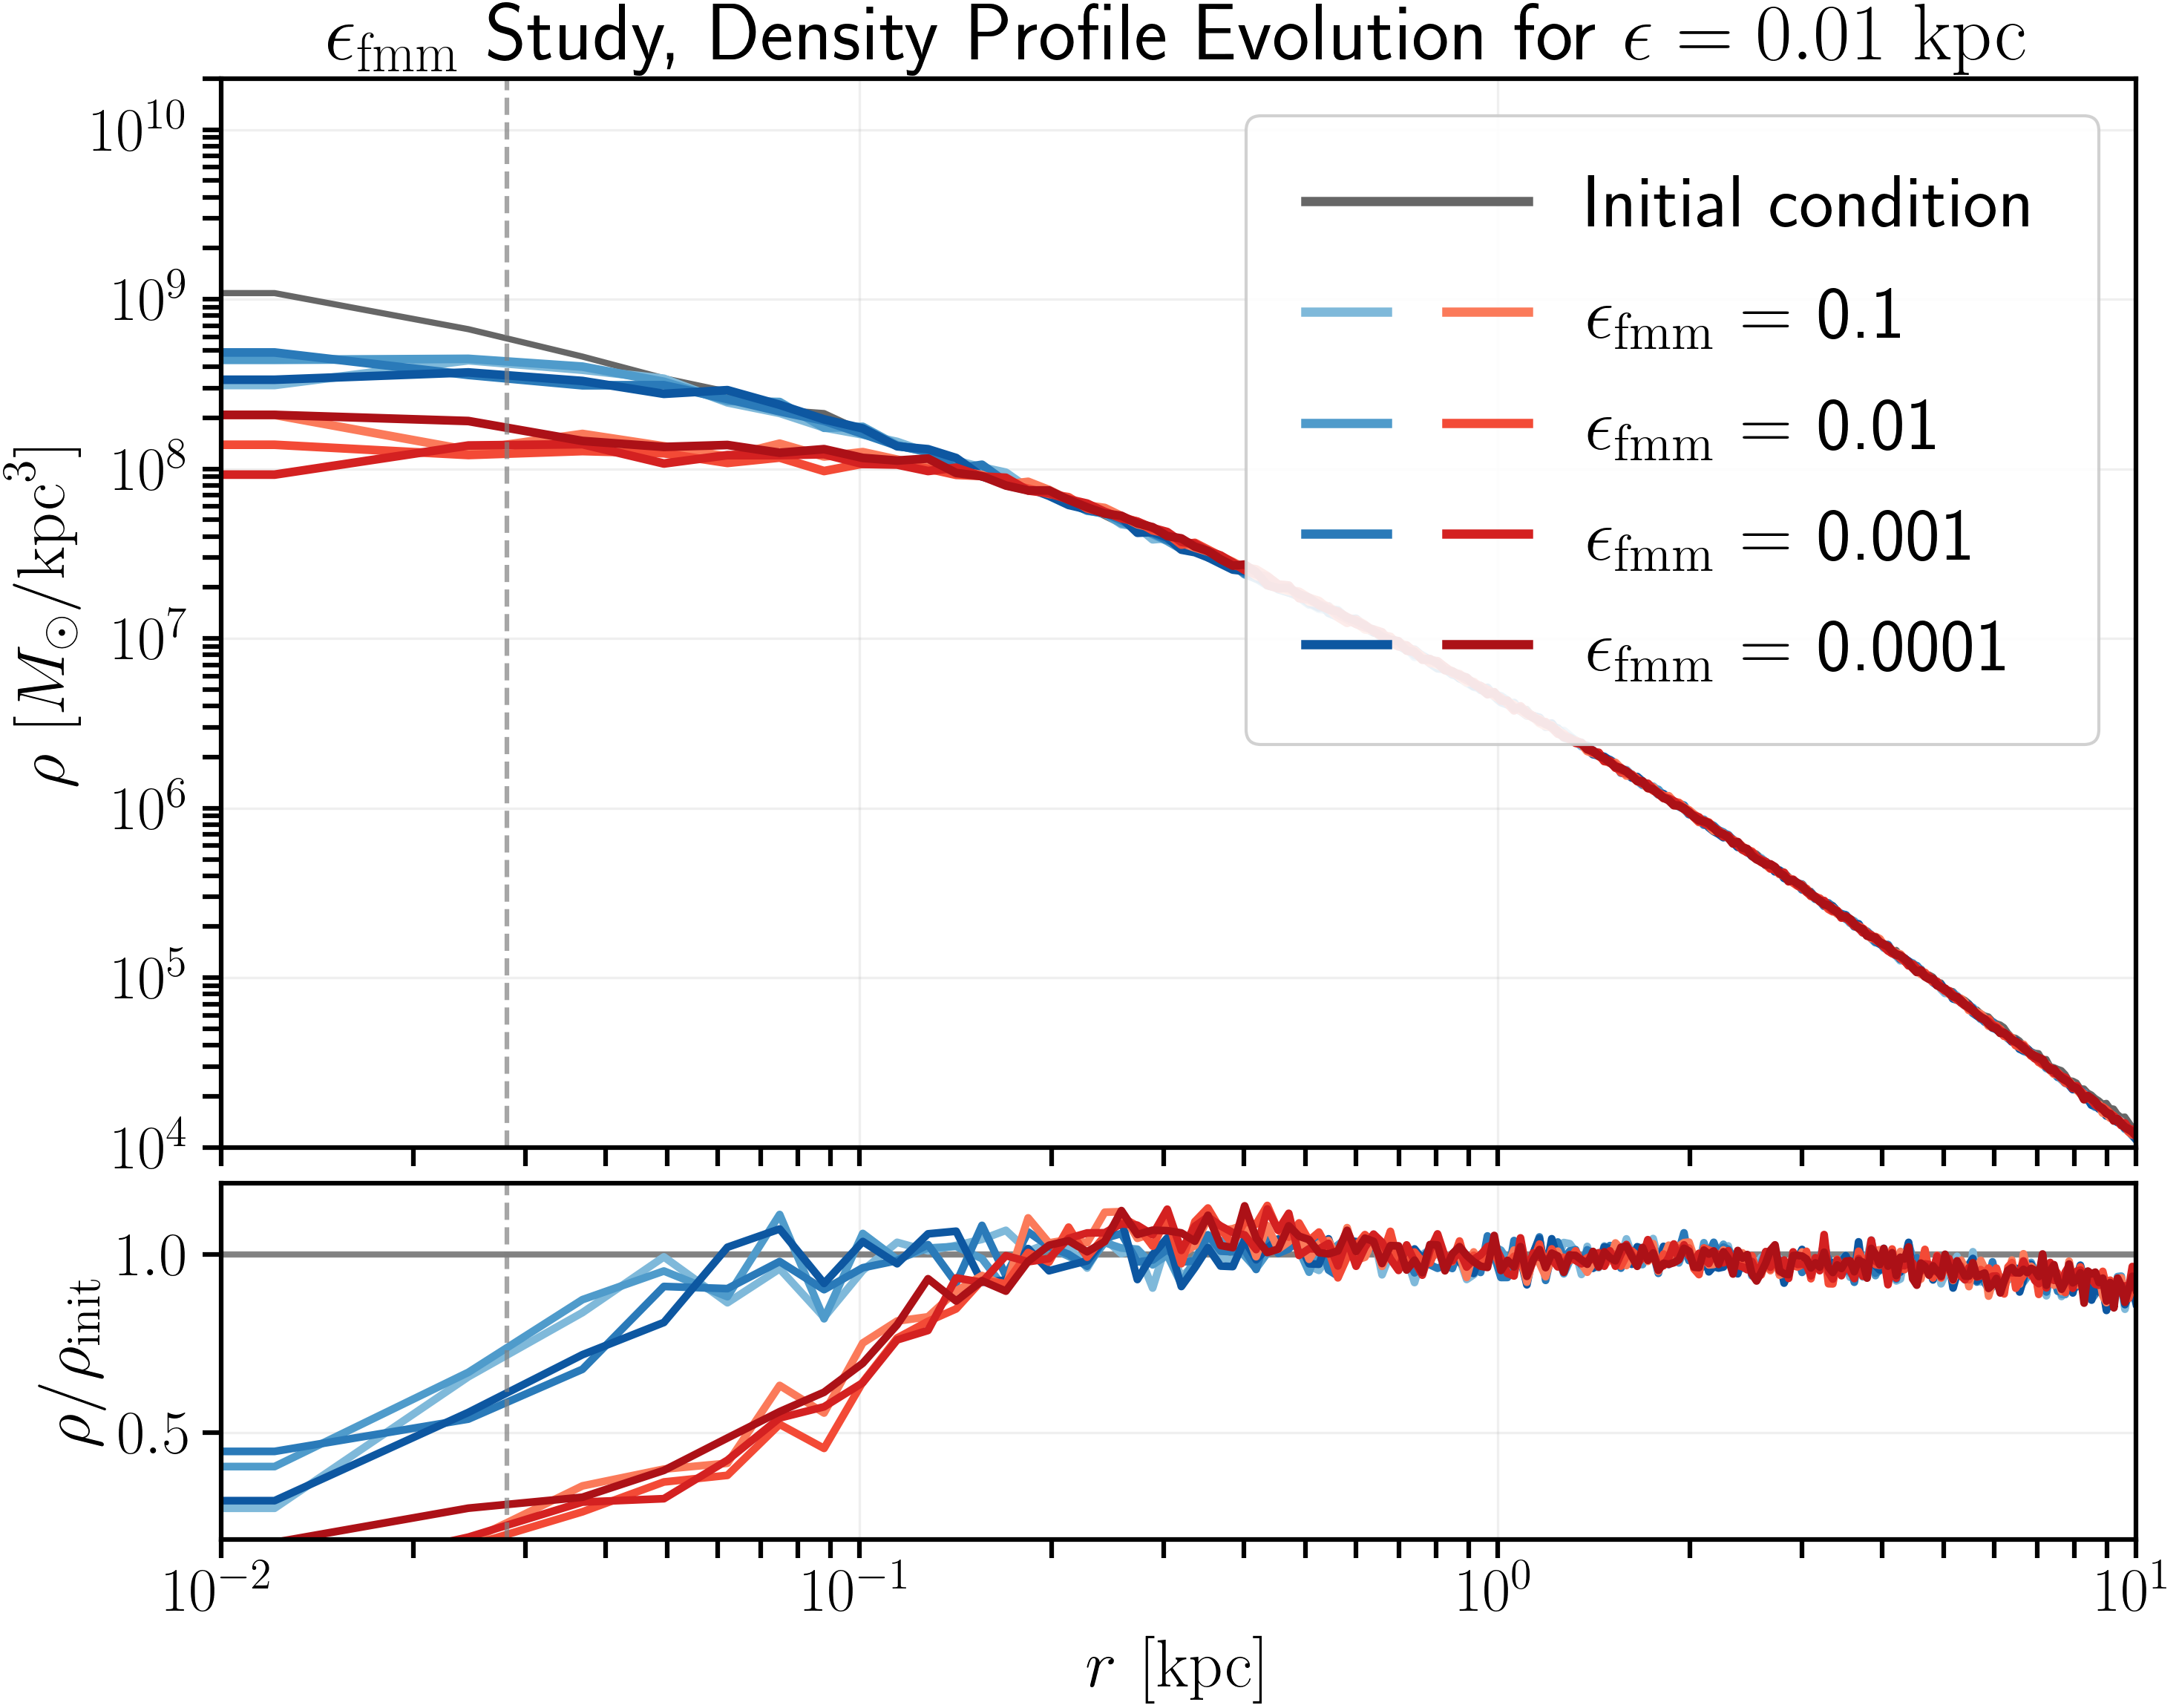
\includegraphics[width=0.48\textwidth]{ch5/img/epsilon_fmm_study.png}}{\fbox{\parbox[c][0.18\textheight][c]{0.48\textwidth}{\centering \textbf{[PLACEHOLDER FIGURE]} $\epsilon_{\mathrm{fmm}}$ study}}}
	\caption{\textbf{[PLACEHOLDER FIGURES]} Parameter-study panels for the self-gravity settings. The final image files will be placed in \texttt{ch5/img}.}
	\label{fig:results_solver}
\end{figure}

The conclusion is that the trend is robust against the standard solver controls. This removes another plausible numerical explanation and strengthens the case for a mechanism tied to the structure of the halo rather than to a single gravity-accuracy parameter.

\section{Cumulative mass and angular momentum}
\label{sec:results_cumulative_mass}

This section is not yet completed.

\textbf{[PLACEHOLDER RESULT]} Here we will quantify whether mass is moving outward from the center, whether $M(<r)$ decreases at small radii, and whether the central angular momentum increases over time.

\textbf{[PLACEHOLDER FIGURE]} Cumulative mass enclosed within radius as a function of time.

\textbf{[PLACEHOLDER FIGURE]} Mass-profile evolution at several snapshots.

\textbf{[PLACEHOLDER FIGURE]} Central angular momentum versus time.

\section{Shell study}
\label{sec:results_shell_study}

This section is not yet completed.

\textbf{[PLACEHOLDER RESULT]} Here we will present the shell-contribution analysis and show why the outer shells matter for the central particle's dynamics.

\textbf{[PLACEHOLDER FIGURE]} Shell contribution to velocity dispersion over time.

\textbf{[PLACEHOLDER FIGURE]} Cumulative contribution by radius.

\section{Truncated NFW}
\label{sec:results_truncated_nfw}

This section is not yet completed.

\textbf{[PLACEHOLDER RESULT]} Here we will compare the standard runs against the truncated-NFW hybrid model.

\textbf{[PLACEHOLDER FIGURE]} Baseline versus truncated-NFW central-density evolution.

\section{Synthesis}
\label{sec:results_synthesis}

This section is not yet completed.

\textbf{[PLACEHOLDER RESULT]} Here we will summarize which explanations have been ruled out and which remain plausible.

\textbf{[PLACEHOLDER FIGURE]} Final synthesis plot or compact summary table of the tests.
